
\noindent\textbf{10. (CRLS 22.3-8)} Mostre um contraexemplo para a conjectura que se existe um caminho de $u$
a $v$ em um grafo orientado $G$, então qualquer \proc{DFS} deve resultar em $d[v] \leq f[u]$.

A figura \ref{fig:7.10-1} mostra um contraexemplo da conjectura. Temos um caminho de $u$ a $v$ no grafo, porém, aplicando a \proc{DFS} a partir de $s$, temos que $d[v] > f[u]$.
\begin{center}
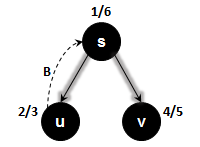
\includegraphics[width=0.28\textwidth]{q7-10.png}
\captionof{figure}{Contraexemplo da conjectura dada.}
\label{fig:7.10-1}
\end{center}